\documentclass[11pt,letterpaper]{article}

% ── Packages ──────────────────────────────────────────────
\usepackage[margin=0.9in,top=0.8in,bottom=0.8in]{geometry}
\usepackage{amsmath,amssymb}
\usepackage{enumitem}
\usepackage{hyperref}
\usepackage[dvipsnames]{xcolor}
\usepackage{microtype}
\usepackage{parskip}
\usepackage{titlesec}
\usepackage{booktabs}
\usepackage{graphicx}
\usepackage{fancyvrb}
\usepackage{tikz}
\usetikzlibrary{arrows.meta,positioning}

% ── Formatting ────────────────────────────────────────────
\hypersetup{colorlinks=true, linkcolor=NavyBlue, citecolor=NavyBlue, urlcolor=NavyBlue}
\titleformat{\section}{\large\bfseries}{\thesection}{1em}{}
\titleformat{\subsection}{\normalsize\bfseries}{\thesubsection}{1em}{}
\setlength{\parskip}{0.6em}

\begin{document}

% ── Title ─────────────────────────────────────────────────
\begin{center}
{\LARGE\bfseries Cross-Patient Neural Speech Decoding}\\[12pt]
{\normalsize Ben Tang \quad\textbar\quad Cogan Lab, Duke University \quad\textbar\quad April 2026}
\end{center}

\medskip\noindent\rule{\textwidth}{0.4pt}\medskip


%% ====================================================================
\section{What Is Shared Across Patients?}
%% ====================================================================

\subsection*{Conserved cortical organization}

Speech motor cortex has a \textbf{conserved somatotopic layout} across all humans: face, jaw, tongue, and larynx representations are arranged in a consistent order along the central sulcus (Breshears 2015, $n{=}33$; Bouchard 2013; Roux 2020). The \textit{ordinal} arrangement is invariant; the \textit{absolute positions} vary by 5--15\,mm between individuals.

We define 16 \textbf{cortical nodes} at atlas-derived positions (Brainnetome, $N{=}40$ HCP subjects) corresponding to known speech-relevant regions. These are the subject-invariant functional units:

\begin{figure}[ht]
\centering
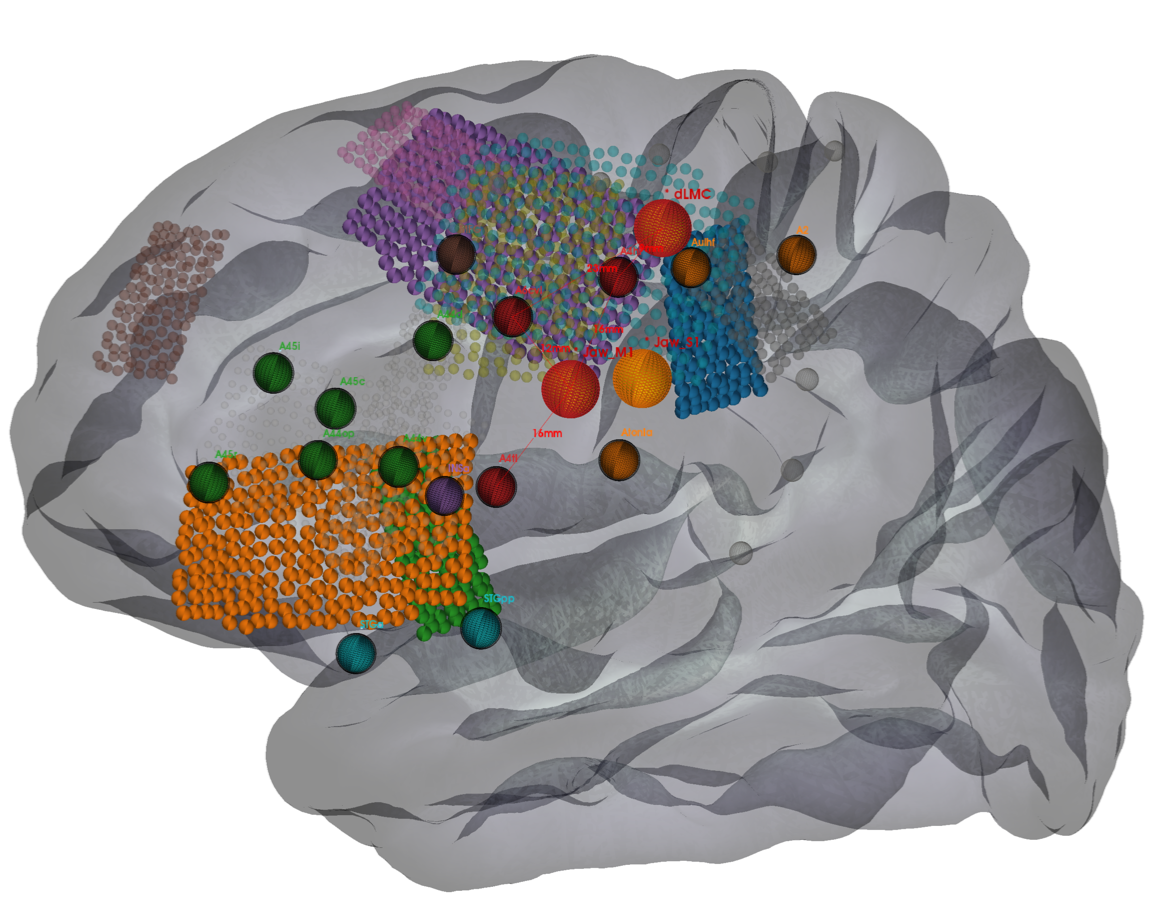
\includegraphics[width=0.45\textwidth]{figures/ve_full_coverage.png}
\caption{16 cortical nodes (large spheres) and patient electrode arrays (small dots). Each patient covers a different subset of nodes.}
\end{figure}

\noindent Key nodes along the motor strip (dorsal $\to$ ventral): \textbf{A4hf} (face M1, MNI $-$49/$-$6/40) $\to$ \textbf{A6cvl} (ventral PMC, $-$49/6/31) $\to$ \textbf{A4tl} (tongue M1, $-$52/2/9). Plus 3 sensory (face/tongue S1, proprioceptive), 6 Broca's (articulatory planning), 2 auditory (self-monitoring), 1 insula, 1 prefrontal. Each node reachable by 3--9 of our 10 patients.

\subsection*{Subject-invariant phoneme dynamics}

Each phoneme activates a \textbf{specific, predictable combination of cortical nodes} determined by articulatory biomechanics:

\begin{itemize}[leftmargin=2em]
\item \textbf{/b/, /p/} (bilabial stops): lip closure $\to$ \textbf{face M1} fires
\item \textbf{/g/, /k/} (velar stops): tongue dorsum raises $\to$ \textbf{tongue M1} fires
\item \textbf{/v/} (labiodental fricative): lower lip to teeth $\to$ \textbf{face M1} fires
\item \textbf{/a/} (open vowel): jaw opening + tongue low $\to$ \textbf{tongue M1} + jaw area
\item \textbf{/i/} (high front vowel): tongue raised front $\to$ \textbf{tongue M1}
\item \textbf{/u/} (high back vowel): tongue raised back + lip rounding $\to$ \textbf{tongue M1} + \textbf{face M1}
\end{itemize}

These node activations follow a conserved temporal cascade: \textbf{Broca's} ($-$200 to $-$50\,ms, planning) $\to$ \textbf{Motor cortex} ($-$50 to +100\,ms, execution) $\to$ \textbf{Somatosensory} (+50 to +200\,ms, feedback) $\to$ \textbf{Auditory} (+100 to +300\,ms, self-monitoring).

\textbf{The ground truth}: what is conserved across patients is (1) the existence and gross positions of cortical nodes representing articulatory muscles, and (2) the spatiotemporal activation sequences across these nodes during phoneme production. A 3-phoneme token like /abe/ produces a characteristic trajectory through the node network --- Broca's plans the sequence, then face M1 fires for /b/, tongue M1 for /a/ and /e/, with sensory and auditory feedback following each.


%% ====================================================================
\section{What Do We Observe?}
%% ====================================================================

We have \textbf{noisy, spatially-sampled observations} of these node activations. Each patient has a $\mu$ECoG electrode array (128 or 256 channels, 1.3--1.7\,mm pitch) pressed against the cortical surface during intra-operative speech. We measure high-gamma activity (HGA, 70--150\,Hz envelope at 200\,Hz) --- a proxy for local cortical population activity.

The physics of this measurement is well-characterized: the signal at each electrode is a \textbf{linear superposition} of cortical sources, contributions \textbf{decay with distance} (${\sim}1/d^2$), and sources beyond ${\sim}$25\,mm are below the noise floor. Crucially, this spatial mapping depends \textbf{only on geometry} --- it does not change based on what the brain is currently doing.

Every patient's array sits in a \textbf{different position} (15--25\,mm offsets, variable rotation). Each array is a partial view of the cortical node network from a different vantage point.


%% ====================================================================
\section{What Must We Learn?}
%% ====================================================================

\subsection*{Per patient (geometry --- \textit{where} things are)}

\begin{enumerate}[leftmargin=2em, itemsep=0.2em]
\item \textbf{Electrode localization error} (6 params): Surgical reconstruction has ${\sim}$4--8\,mm systematic rigid-body error. Learn translation $\Delta$ + rotation $\omega$, clamped ($\|\Delta\| \leq 15$\,mm, $\|\omega\| \leq 0.15$\,rad).

\item \textbf{Individual cortical node positions} (48 params): Individual anatomy varies by 5--15\,mm from atlas. Each of 16 nodes gets a learned offset $\delta_l \in \mathbb{R}^3$, clamped $\leq$15\,mm. Initialized at zero (trust the atlas).

\item \textbf{Signal gain and offset} (128 params): Electrode impedance varies. Per-channel scale (positive via softplus) and offset. Initialized from channel statistics.
\end{enumerate}

\textbf{Total: 182 parameters per patient.} Comparable cross-patient iEEG systems (seegnificant, MIBRAIN, BarISTA) use per-subject heads or region prototypes with similar or larger per-patient footprints, or no per-patient adaptation at all.

\subsection*{Shared (dynamics --- \textit{what} things mean)}

\textbf{Spatiotemporal activation patterns on cortical nodes $\to$ which phoneme sequence.} Given correctly-positioned nodes with correctly-calibrated signals pooled into them, the 16-node network dynamics encode the phoneme. Same mapping for every patient --- determined by conserved cortical organization, not individual anatomy.


%% ====================================================================
\section{What Architecture Does This Ask For?}
%% ====================================================================

Each component follows directly from the physics:

\begin{Verbatim}[frame=single, fontsize=\small]
Raw electrode HGA (N_i electrodes x T time steps)
  -> Temporal binning: Conv1d(1->d, k=10, s=10)        [200Hz -> 20Hz]
  -> Per-patient calibration:                           [182 params/pt]
       softplus(s) * x + b   (gain/offset, positive)
       correct electrode positions (6 params: rigid)
       correct node positions (48 params: individual somatotopy)
  -> Spatial pooling into 16 cortical nodes             [physics-derived]
       Wendland kernel, distance-weighted, compact support
  -> [Node self-attention + Temporal self-attention] x 2  [learns dynamics]
  -> AR decoder: predict phoneme 1, 2, 3 + beam search   [52 valid tokens]
\end{Verbatim}

\subsection*{Spatial pooling}

Each node computes a weighted average of nearby electrode signals, where the weights depend only on distance --- electrodes closer to the node contribute more, and electrodes beyond a learned radius $R$ contribute nothing:
\begin{equation}
z_{\text{node}} = \sum_{j} \underbrace{\frac{w(\text{dist}_{j},\, R)}{\sum_{j'} w(\text{dist}_{j'},\, R)}}_{\text{distance-only weights}} \cdot \underbrace{(x_j\, W)}_{\text{learned features}}
\end{equation}
Multiple pooling heads operate at different radii (tight ${\sim}$10\,mm for focal activity, broad ${\sim}$25\,mm for regional), each extracting different learned features before averaging.

\subsection*{Parameter budget}

\begin{table}[ht]\centering\small
\begin{tabular}{@{}lrl@{}}
\toprule
\textbf{Component} & \textbf{Params} & \textbf{Note} \\
\midrule
Conv1d + feature projections & ${\sim}$5K & Shared: temporal features \\
Spatial pooling (Wendland) & $H$ scalars & Shared: learned $R_h$ per head \\
Spatiotemporal blocks ($\times$2) & ${\sim}$132K & Shared: node dynamics \\
AR decoder & ${\sim}$4K & Shared: phoneme sequence \\
\midrule
Gain/offset (softplus$(s) \odot x + b$) & 128/pt & Per-patient: impedance \\
Electrode correction ($\Delta$, $\omega$) & 6/pt & Per-patient: registration error \\
Node offsets ($\delta_l$) & 48/pt & Per-patient: individual somatotopy \\
\midrule
\textbf{Total shared} & $\mathbf{{\sim}141}$\textbf{K} & \\
\textbf{Total per-patient} & \textbf{182} & \\
\bottomrule
\end{tabular}
\end{table}

\subsection*{Immediate next steps}

\begin{enumerate}[leftmargin=2em]
\item \textbf{Scale data} (highest priority) --- to learn the shared spatiotemporal dynamics we need a foundation of data. Could request chronic ECoG speech data from Flinker/Chen (NYU, 48 patients) and/or Chang (UCSF, ${\sim}$15--25 patients)
\item \textbf{Nonlinear MNI normalization} --- current electrode transform is linear-only (${\sim}$5--15\,mm residual error); if T1 MRIs exist, ANTs SyN could halve this
\item \textbf{Implementation} --- architecture is designed; target ${\sim}$2 weeks to first training run on DCC
\end{enumerate}


\end{document}
